\documentclass[a4paper,fleqn]{cas-sc}

\usepackage[authoryear]{natbib}
\usepackage{amsmath,amssymb}
\usepackage{booktabs}
\usepackage{array}
\usepackage{graphicx}
\usepackage{tikz}
\usepackage{pgfplots}
\pgfplotsset{compat=1.18}
\usepackage{url}
\usepackage{hyperref}

\begin{document}

% ============================================================================
% TITLE AND ABSTRACT
% ============================================================================

\title[short title]{SAT vs.\ CP-SAT vs.\ Classical Backtracking for Generalized Sudoku: An Empirical Benchmark}

\author[1]{[Author Name]}\ead{[email]}

\affiliation[1]{
    organization=[Institution],
    addressline=[Address],
    city=[City],
    postcode=[Postal Code],
    state=[State],
    country=[Country]
}

\begin{abstract}

This paper presents an empirical comparison of three solver families---SAT, constraint programming (CP-SAT), and classical backtracking---on a shared benchmark of generalized Sudoku instances. We evaluate seven PySAT configurations spanning five At-Most-One (AMO) encodings (pairwise, sequential counter, binary, commander, product) across three CDCL backends (CaDiCaL 1.5.3, Glucose 4, MiniSat 2.2), Google OR-Tools CP-SAT, and an optimized backtracking implementation using minimum-remaining-values (MRV) cell selection with forward checking. The benchmark comprises 120 Sudoku instances across grid sizes \(N \in \{9, 36, 81\}\) and clue-removal ratios \(r \in \{0.5, 0.9\}\), with 20 instances per stratum, generated from a single seed (42). Every solver run is subject to a 10.0-second wall-clock timeout, a 60\% available-memory resource guard, and independent solution verification. Across 1{,}000 attempted runs (760 SAT, 120 CP-SAT, 120 backtracking), SAT solvers produce 431 valid solutions (56.71\%), CP-SAT produces 64 (53.33\%), and backtracking produces 40 (33.33\%), all independently verified with zero invalid solutions. Both SAT and CP-SAT achieve 100\% solve rates on \(9\times9\) instances and zero valid solutions on \(81\times81\) within the timeout. On \(36\times36\) at \(r=0.5\), solve rates fall below 21\% for all families. We find no evidence of universal superiority: pooling seven SAT configurations gives SAT a different aggregation structure than the two single-configuration baselines, and pairwise/binary SAT encodings are predeclared excluded at \(N=81\) by the memory guard, leaving their performance at that size unknown. No confidence intervals, hypothesis tests, or replications are reported; all findings are descriptive and timeout-censored.

\end{abstract}

\begin{keywords}
Sudoku \sep SAT encoding \sep CP-SAT \sep classical backtracking \sep constraint programming \sep benchmarking \sep AMO encoding
\end{keywords}

\maketitle

% ============================================================================
% 1. INTRODUCTION
% ============================================================================

\section{Introduction}

Sudoku is a number-placement constraint satisfaction problem in which an \(N\times N\) grid (with \(N=k^2\) for box size \(k\)) must be completed so that every row, column, and \(k\times k\) box contains each digit \(1,\dots,N\) exactly once, consistent with pre-filled clue cells. The decision version of Sudoku is NP-complete \citep{yato2003sudoku}, which makes it a natural benchmark for comparing combinatorial search paradigms. Despite its simple rules, Sudoku instances exhibit wide variation in solving difficulty depending on grid size and clue density, and no single solving approach dominates across all regimes.

Three solving families are widely used in practice. Boolean satisfiability (SAT) solvers encode Sudoku as a conjunctive normal form formula using one-hot Boolean variables \(x[r,c,v]\) and exactly-one (at-least-one plus at-most-one) constraints per cell, row, column, and box. The choice of At-Most-One (AMO) encoding---pairwise, sequential counter, binary, commander, or product---materially affects formula size and propagation strength, and modern CDCL backends differ in restart, conflict-analysis, and clause-deletion heuristics. Constraint programming solvers such as OR-Tools CP-SAT model Sudoku directly with integer variables in domain \(1..N\) and global all-different constraints, combining constraint propagation with CDCL-style clause learning. Classical backtracking explores partial assignments with variable and value ordering heuristics, optionally augmented with forward checking or arc consistency.

Prior work has studied SAT encodings for Sudoku \citep{lynce2006sudoku}, AMO encoding trade-offs \citep{sinz2005towards,nguyen2020empirical,hn2013efficient,klieber2007effective,chen2010new,frisch2010sat}, and constraint programming for Sudoku \citep{simonis2005sudoku,aaai2007interactive}. However, we are not aware of prior work that directly compares five AMO encodings across three CDCL backends, CP-SAT, and classical backtracking on identical generalized Sudoku instances spanning \(N \in \{9, 36, 81\}\), with independent solution validation on every returned candidate.

This study addresses three experimental questions:

\begin{enumerate}
    \item \textbf{RQ1:} How do five SAT AMO encodings and three CDCL backends compare in valid solve rate and solve time on identical Sudoku instances?
    \item \textbf{RQ2:} How do SAT-based solvers compare with OR-Tools CP-SAT and classical backtracking in valid solve rate and solve time?
    \item \textbf{RQ3:} How do grid size (\(N \in \{9, 36, 81\}\)) and clue-removal ratio (\(r \in \{0.5, 0.9\}\)) relate to success rate and solve time across solver families?
\end{enumerate}

The defensible contributions of this paper are: (i) a documented benchmark of 1{,}000 attempted solver runs across three solver families and twelve problem strata, with raw results and an independent validator; (ii) descriptive evidence that SAT and CP-SAT achieve comparable valid solve rates (56.71\% vs.\ 53.33\%) on shared instances, while classical backtracking solves 40 of 120 instances, all confined to \(N=9\); (iii) documentation of a hardness cliff at \(N=36, r=0.5\) (solve rates below 21\% for all families) and intractability at \(N=81\) within a 10-second timeout; and (iv) explicit accounting of predeclared memory-guard exclusions, live resource-guard rejections, and timeout censoring, which limit the inferential strength of all comparisons. We make no claim of universal superiority for any solver family, no claim of statistical significance, and no generalization beyond the tested dataset.

% ============================================================================
% 2. RELATED WORK
% ============================================================================

\section{Related Work}

\subsection{SAT formulations for Sudoku}

\citet{lynce2006sudoku} introduced the first SAT encodings for Sudoku, proposing minimal and extended CNF formulations using one-hot Boolean variables with exactly-one constraints per cell, row, column, and box. They report that unit propagation on the extended encoding can solve approximately half of hard \(9\times9\) puzzles without search. This work established the one-hot Boolean formulation---\(N^3\) primary variables and \(4N^2\) exactly-one groups---that underlies all SAT configurations evaluated here.

\citet{kwon2016optimized} presented an optimized CNF encoding for Sudoku aimed at reducing clause count for larger puzzles. Full bibliographic details (venue, year, DOI) could not be verified against a primary source; this reference is cited for context only and no technical claim in this paper depends on it.

\subsection{At-Most-One encodings}

Five AMO encodings are implemented and evaluated. \citet{sinz2005towards} introduced the sequential counter encoding for Boolean cardinality constraints, using \(O(n)\) auxiliary variables and \(O(n)\) clauses for an at-most-one constraint over \(n\) literals; this is the basis of the sequential encoding in \texttt{sat.py}. \citet{klieber2007effective} proposed the commander encoding, which partitions literals into subgroups with commander variables and a group-size parameter \(b\); the implementation uses \(b=4\). Full bibliographic verification of \citet{klieber2007effective} against a primary source is incomplete; it is referenced as a secondary citation in \citet{hn2013efficient}. \citet{chen2010new} introduced the product encoding, arranging literals in a two-dimensional grid with row and column indicator variables; full bibliographic verification against a primary source is incomplete. \citet{frisch2010sat} presented binary/bitwise at-most-one encodings using \(\lceil\log_2 n\rceil\) auxiliary variables. Full bibliographic verification against a primary source is incomplete.

\citet{nguyen2020empirical} provided an empirical comparison of AMO encodings (pairwise, sequential, binary, commander, product, bimander) across three SAT solvers on generic benchmarks, finding that encoding choice has a measurable impact on solver performance. Our study applies the same five encodings to Sudoku specifically, across multiple grid sizes and three CDCL backends, with independent solution validation. \citet{hn2013efficient} is a technical survey of AMO encodings with clause and variable count comparisons; it provides the complexity table used in Section 3 but reports no empirical Sudoku runtime results.

\subsection{Constraint programming and CP-SAT}

\citet{simonis2005sudoku} modeled Sudoku as a constraint satisfaction problem using all-different constraints on rows, columns, and boxes, contrasting 27 arity-9 all-different constraints with 810 binary inequality constraints. \citet{aaai2007interactive} presented an interactive constraint-based Sudoku solver and confirmed that Sudoku is NP-complete via \citet{yato2003sudoku}; this work is educational/interactive in focus and reports no cross-solver benchmarking. OR-Tools CP-SAT \citep{ortools2026} is a hybrid constraint-programming solver built on a CDCL SAT engine and enriched with MIP techniques; it accepts integer decision variables and global all-different constraints directly. The CP-SAT configuration evaluated here uses \(N^2\) integer variables in domain \(1..N\) with all-different constraints per row, column, and box, plus unit equality constraints for clues.

\subsection{Classical backtracking}

Classical backtracking for Sudoku selects an unassigned variable, tries candidate values, and backtracks on contradiction. The implementation evaluated here uses minimum-remaining-values (MRV) cell selection, forward checking after each assignment, and optional AC-3 propagation over binary peer inequalities (disabled in the benchmark runs). Candidates are tried in ascending order; MRV ties break on lowest cell index (row-major). No least-constraining-value (LCV) heuristic and no degree heuristic are implemented. Source inspection confirms these design choices; see Section 3 and \texttt{src/sudoku\_solver/backtracking.py}.

\subsection{Solver benchmarking and reproducibility}

\citet{nguyen2020empirical} and \citet{sheng2025reencoding} discuss encoding-size versus runtime trade-offs and the importance of empirical evaluation over theoretical clause counts alone. Full bibliographic verification of \citet{sheng2025reencoding} against a primary source is incomplete. This study contributes an empirical Sudoku-specific comparison but shares the limitations of single-seed, single-run benchmarks: no confidence intervals, no replication, and timeout-censored runtimes preclude inferential claims (Sections 5--7).

% ============================================================================
% 3. PROBLEM FORMULATION AND SOLVER METHODS
% ============================================================================

\section{Problem Formulation and Solver Methods}

\subsection{Generalized \(N\times N\) Sudoku}

A Sudoku puzzle of size \(N\times N\), where \(N=k^2\) for box size \(k\), consists of an \(N\times N\) grid with some cells pre-filled (clues) and the remainder empty. The objective is to fill every empty cell with a digit from \(1\) to \(N\) such that:
\begin{enumerate}
    \item each row contains each digit exactly once;
    \item each column contains each digit exactly once;
    \item each \(k\times k\) box contains each digit exactly once;
    \item every pre-filled clue matches the corresponding cell in the solution.
\end{enumerate}

A solution is valid if it satisfies all constraints. Solution uniqueness is not required: any valid completion matching the clues counts as correct, as implemented in \texttt{is\_valid\_solution\_for\_puzzle} (\texttt{src/sudoku/validator.py}).

\subsection{SAT formulation and AMO encodings}

The SAT model uses \(N^3\) one-hot Boolean variables \(x[r,c,v]\), where \(x[r,c,v]=1\) iff cell \((r,c)\) contains digit \(v\), mapped to 1-based index \(r\cdot N^2 + c\cdot N + v\). The constraints are:
\begin{enumerate}
    \item \textbf{Cell exactly-one}: each cell contains exactly one digit (\(N^2\) groups of size \(N\)).
    \item \textbf{Row exactly-one}: each digit occurs once per row (\(N^2\) groups).
    \item \textbf{Column exactly-one}: each digit occurs once per column (\(N^2\) groups).
    \item \textbf{Box exactly-one}: each digit occurs once per box (\(N^2\) groups).
    \item \textbf{Clues}: positive unit clauses for pre-filled cells.
\end{enumerate}

There are \(4N^2\) exactly-one groups in total. Each group is encoded as one at-least-one (ALO) clause plus one at-most-one (AMO) encoding chosen from five alternatives implemented in \texttt{src/sudoku/solvers/sat.py}:

\begin{itemize}
    \item \textbf{Pairwise}: forbids every pair of literals in the group; \(0\) auxiliary variables, \(N(N-1)/2\) clauses per group, \(O(N^2)\) clauses per group.
    \item \textbf{Sequential counter} (\citeyear{sinz2005towards}): prefix variables record whether a literal in the prefix is true; \(N-1\) auxiliary variables, \(O(N)\) clauses per group.
    \item \textbf{Binary} (\citeyear{frisch2010sat}): each literal forces a distinct binary bit pattern on auxiliary variables; \(\lceil\log_2 N\rceil\) auxiliary variables, \(O(N\log N)\) clauses per group.
    \item \textbf{Commander} (\citeyear{klieber2007effective}): literals are partitioned into subgroups of size \(b\) (default \(b=4\)) with commander variables; \(\lceil N/b\rceil\) auxiliary variables per group.
    \item \textbf{Product} (\citeyear{chen2010new}): literals are arranged in a 2D grid with row and column indicator variables; approximately \(\lceil\sqrt{N}\rceil + \lceil N/\lceil\sqrt{N}\rceil\rceil\) auxiliary variables per group.
\end{itemize}

Clue cells are encoded as positive unit clauses. PySAT CDCL backends evaluated are CaDiCaL 1.5.3, Glucose 4, and MiniSat 2.2, each invoked through the PySAT \texttt{Solver} interface with bootstrapped clauses. PySAT's \texttt{solve()} does not accept a wall-clock timeout directly; the 10.0-second limit is enforced externally by the subprocess runner via SIGKILL (\texttt{src/sudoku/bench/runner.py}).

\subsection{CP-SAT formulation}

The CP-SAT model uses \(N^2\) integer decision variables \(x[r,c] \in \{1,\dots,N\}\) with all-different constraints per row, column, and box, plus unit equality constraints for clues. OR-Tools CP-SAT combines constraint propagation with CDCL-style conflict analysis. The solver parameter \texttt{max\_time\_in\_seconds} is set to the 10.0-second timeout, and \texttt{num\_workers} is set to 1 (\texttt{src/sudoku/solvers/cpsat.py}).

\subsection{Classical backtracking}

The backtracking solver (\texttt{src/sudoku\_solver/backtracking.py}) maintains a domain of candidate values for each cell, initialized to \(\{1,\dots,N\}\) and narrowed by clues. It implements:
\begin{itemize}
    \item \textbf{MRV cell selection}: the unassigned cell with the fewest remaining candidates is chosen; ties break on lowest cell index (row-major); a cell with an empty domain is returned immediately as a contradiction.
    \item \textbf{Forward checking}: after assigning a value, that value is removed from the domains of all peer cells (sharing a row, column, or box); an emptied domain fails the branch.
    \item \textbf{Optional AC-3}: arc consistency over binary peer inequalities is available via \texttt{use\_ac3}, but is disabled in the benchmark runs (\texttt{use\_ac3=False}); the docstring notes that AC-3 on binary inequalities is weaker than generalized arc consistency on all-different constraints.
    \item \textbf{Depth-first search}: candidates are tried in ascending order; each decision narrows the decision cell's domain to a singleton, propagates, recurses, and restores on failure.
    \item \textbf{Timeout}: the search aborts once a wall-clock deadline is reached and returns timeout status.
\end{itemize}

Source inspection confirms that \textbf{no least-constraining-value (LCV) heuristic and no degree heuristic are implemented}; candidates are sorted ascending and MRV ties break deterministically on cell index. The benchmark invokes the solver with \texttt{use\_ac3=False} and \texttt{randomize=False} (\texttt{src/sudoku/bench/runner.py:run\_solver\_in\_process}).

\subsection{Solver configurations}

Eight configurations were in the primary benchmark matrix: seven SAT configurations and one CP-SAT configuration. Table \ref{tab:configs} lists them. Gurobi and CPLEX adapters exist in the codebase but were not executed due to commercial license restrictions and are excluded from this study. The backtracking solver exists in the codebase and was invoked in a preliminary run (\texttt{full\_v1}), but its results are reported separately from \texttt{data/results/backtracking\_results.csv} (Section 5); see Section 7 for the data-consistency note.

\begin{table}[htbp]
\centering
\caption{Solver configurations in the primary benchmark.}
\label{tab:configs}
\small
\begin{tabular}{lllll}
\toprule
Label & Family & Encoding & Backend & Threads \\
\midrule
sat\_pairwise\_cadical153 & SAT & pairwise & cadical153 & 1 \\
sat\_sequential\_cadical153 & SAT & sequential & cadical153 & 1 \\
sat\_binary\_cadical153 & SAT & binary & cadical153 & 1 \\
sat\_commander\_cadical153 & SAT & commander (\(b=4\)) & cadical153 & 1 \\
sat\_product\_cadical153 & SAT & product & cadical153 & 1 \\
sat\_sequential\_glucose4 & SAT & sequential & glucose4 & 1 \\
sat\_sequential\_minisat22 & SAT & sequential & minisat22 & 1 \\
cpsat & CP-SAT & --- & ortools-cpsat & 1 \\
\bottomrule
\end{tabular}
\end{table}

% ============================================================================
% 4. EXPERIMENTAL DESIGN
% ============================================================================

\section{Experimental Design}

\subsection{Dataset}

The benchmark uses 120 Sudoku instances spanning six difficulty strata: grid sizes \(N \in \{9, 36, 81\}\) (box sizes \(k \in \{3, 6, 9\}\)) and clue-removal ratios \(r \in \{0.5, 0.9\}\), with 20 instances per stratum. These details are confirmed by \texttt{data/dataset\_info.json} (base seed 42, generator version gen-v1, 20 puzzles per pair, 6 pairs, 120 total puzzles) and \texttt{data/manifest.csv}.

Puzzle generation (\texttt{src/sudoku/generator.py}, gen-v1): construct a valid complete grid from the base pattern \((k\cdot(r \bmod k) + r \div k + c) \bmod N + 1\); apply seeded validity-preserving transformations (row permutations within bands, column permutations within stacks, band/stack permutation, optional transpose, digit relabeling); validate the complete grid; remove \(n_\text{remove} = \text{round\_half\_up}(r \times N^2)\) cells; validate the puzzle against the reference solution with \texttt{is\_valid\_puzzle}. Puzzles are not guaranteed to have unique solutions; any valid completion matching clues counts as correct.

The realized removal ratios deviate slightly from requested values due to \texttt{round\_half\_up} and cell-count quantization (e.g., \(N=9, r=0.5\) realizes as \(0.50617\) with 40 clues; \(N=81, r=0.9\) realizes as \(0.90002\) with 656 clues). All puzzles are loaded from stored files; no puzzle regeneration occurs during benchmarking.

Generator limitations (from source documentation): puzzles are sampled from the automorphism equivalence orbit of the standard base pattern, not uniformly from all valid Sudoku grids; removal ratio is an experimental condition, not a difficulty label; only two ratios are tested.

\subsection{Solver configurations, timeout, and resource guard}

Each run executes in an isolated subprocess (\texttt{subprocess.Popen} with \texttt{start\_new\_session=True}) under a 10.0-second wall-clock timeout enforced by SIGKILL via the process monitor. A resource guard estimates CNF build memory for SAT encodings: \(\text{estimated\_bytes} = \text{clauses} \times \text{bytes\_per\_clause}\); if this exceeds \(0.60 \times \text{available RAM}\), the run is recorded as \texttt{BUILD\_FAIL} with \texttt{stats.predeclared\_exclusion=true} and is \emph{not} counted as an attempted run. The guard affects \(N=81\) SAT pairwise and binary encodings only (80 predeclared exclusions total: 40 pairwise + 40 binary across both \(N=81\) strata). One live resource-guard rejection occurred during execution (commander at \(N=81, r=0.5\)); this is counted as an attempted run but not as a valid solution.

Peak RSS is tracked via psutil sampling at 20 ms intervals and \texttt{resource.ru\_maxrss}. Every returned solution is independently verified by \texttt{is\_valid\_solution\_for\_puzzle} (\texttt{src/sudoku/validator.py}), which checks that the candidate is a complete legal grid and matches every clue. A run counts as \texttt{SOLVED\_VALID} only if the solution passes validation.

\subsection{Timing metrics}

Three timing fields are recorded: \texttt{t\_build} (model construction), \texttt{t\_solve} (pure solver solve time), and \texttt{t\_total} (end-to-end, including build, solve, extraction, and validation). For timed-out runs, \texttt{t\_total} is the wall-clock elapsed time until SIGKILL. Medians and percentiles reported in Section 5 are computed over successful (\texttt{SOLVED\_VALID}) runs only.

\subsection{Environment}

Python 3.14.8 is confirmed by \texttt{data/dataset\_info.json}. PySAT, OR-Tools, and psutil are used. Gurobi and CPLEX adapters exist but were not executed (license restrictions). \textbf{Hardware specifications (CPU, RAM, operating system) are not recorded}; \texttt{full\_v1\_run\_info.json} reports \texttt{environment\_lock\_present=false}, and no environment lock file is present in the repository. Exact solver version pins beyond backend names (cadical153, glucose4, minisat22) are not recorded. These gaps are disclosed in Section 7.

\subsection{Single-seed design and lack of replication}

All puzzles are generated from base seed 42. One run is performed per instance per configuration; there is no replication across seeds or runs. Consequently, no variance estimates, confidence intervals, or hypothesis tests are available. All statistics in Section 5 are descriptive, computed from single measurements, and are timeout-censored (timeouts contribute to denominators but have no finite solve time).

\begin{figure}[htbp]
\centering
% ============================================================================
% Figure 5: Experimental workflow diagram (Optimized layout)
% ============================================================================
\begin{tikzpicture}[
  font=\sffamily\footnotesize,
  node distance=0.8cm and 0.5cm,
  box/.style={draw, rounded corners=2pt, fill=blue!8, minimum width=2.4cm, minimum height=0.7cm, align=center, font=\sffamily\scriptsize},
  decbox/.style={draw, rounded corners=2pt, fill=orange!12, minimum width=2.4cm, minimum height=0.7cm, align=center, font=\sffamily\scriptsize},
  outbox/.style={draw, rounded corners=2pt, fill=green!10, minimum width=2.4cm, minimum height=0.7cm, align=center, font=\sffamily\scriptsize},
  exclbox/.style={draw, rounded corners=2pt, fill=red!8, minimum width=2.4cm, minimum height=0.7cm, align=center, font=\sffamily\scriptsize},
  arr/.style={->, thick, shorten >=1pt, shorten <=1pt},
  every node/.append style={align=center}
]
\node[box] (dataset) {Dataset\\ 120 Sudoku instances\\ $N\in\{9,36,81\}$, $r\in\{0.5,0.9\}$\\ 20 per stratum, seed 42};
\node[box, below=1.2cm of dataset, xshift=-3.1cm] (sat) {SAT configs\\ 7 configs: 5 AMO encodings\\ across 3 CDCL backends};
\node[box, below=1.2cm of dataset] (cpsat) {CP-SAT\\ OR-Tools, 1 config\\ $N^2$ int vars + all-diff};
\node[box, below=1.2cm of dataset, xshift=3.1cm] (bt) {Backtracking\\ 1 config, MRV + fwd checking};
\node[decbox, below=0.8cm of sat] (sat_guard) {Memory resource guard\\ 60\% available RAM\\ (pre-execution estimate)};
\node[decbox, below=0.8cm of cpsat] (cpsat_guard) {Memory resource guard\\ 60\% available RAM\\ (no exclusion triggered)};
\node[decbox, below=0.8cm of bt] (bt_guard) {Memory resource guard\\ 60\% available RAM\\ (no exclusion triggered)};

% Predeclared exclusions: placed to the LEFT of the SAT guard (was below it, overlapping the run box/arrows)
\node[exclbox, left=0.6cm of sat_guard] (excluded) {Predeclared excl.\\ pairwise + binary\\ at $N=81$ (80 runs)\\ not attempted};

\node[box, below=1.8cm of cpsat_guard, minimum width=6.5cm] (run) {Isolated subprocess run per (puzzle, config)\\ wall-clock timeout 10.0 s};
\node[outbox, below=0.8cm of run, minimum width=6.5cm] (valid) {Independent validation (\texttt{is\_valid\_solution\_for\_puzzle})\\ complete grid + clue match};
\node[box, below=0.8cm of valid, minimum width=6.5cm] (status) {Run statuses: SOLVED\_VALID / TIMEOUT /\\ BUILD\_FAIL / SOLVER\_ERROR / RESOURCE\_GUARD\_LIVE};
\node[outbox, below=0.8cm of status, minimum width=6.5cm] (analysis) {Result analysis\\ valid rate, timeout rate, median runtime, tables/figures};

\draw[arr] (dataset.south) -- (cpsat.north);
\draw[arr] (dataset.south) -| (sat.north);
\draw[arr] (dataset.south) -| (bt.north);
\draw[arr] (sat.south) -- (sat_guard.north);
\draw[arr] (cpsat.south) -- (cpsat_guard.north);
\draw[arr] (bt.south) -- (bt_guard.north);
\draw[arr, dashed] (sat_guard.west) -- (excluded.east);
\draw[arr] (sat_guard.south) -- ([xshift=-1.5cm]run.north);
\draw[arr] (cpsat_guard.south) -- (run.north);
\draw[arr] (bt_guard.south) -- ([xshift=1.5cm]run.north);
\draw[arr] (run) -- (valid);
\draw[arr] (valid) -- (status);
\draw[arr] (status) -- (analysis);
\end{tikzpicture}
\caption{Experimental workflow. Twelve puzzles per stratum are paired with solver configurations (seven SAT, one CP-SAT, one backtracking). Each run executes under a 10.0-second wall-clock timeout and a 60\% available-memory resource guard; pairwise and binary SAT encodings at \(N=81\) are predeclared excluded by the guard. Every returned solution is independently verified by \texttt{is\_valid\_solution\_for\_puzzle} before a run is classified as \texttt{SOLVED\_VALID}. Result statuses feed the aggregate, per-configuration, and stratified analyses in Section 5. Excluded runs are not attempted and therefore do not enter the run or validation stages.}
\label{fig:workflow}
\end{figure}

% ============================================================================
% 5. RESULTS
% ============================================================================

\section{Results}

\subsection{Aggregate solver-family comparison}

Table \ref{tab:t1} reports the aggregate comparison across the three solver families. Denominators strictly exclude predeclared memory-guard exclusions. Valid-solution rate is \(\text{Valid Solutions}/\text{Attempted Runs}\). Timeout rate is timeouts divided by attempted runs.

\begin{table}[htbp]
\centering
\caption{Aggregate solver-family comparison. Denominators exclude 80 predeclared SAT memory-guard exclusions. Valid rate and timeout rate are computed over attempted runs. Median solve time is over successful runs only.}
\label{tab:t1}
\small
\begin{tabular}{lccc}
\toprule
Metric & SAT (7 configs) & CP-SAT (1 config) & Backtracking (1 config) \\
\midrule
Solver configurations & 7 & 1 & 1 \\
Recorded matrix cells & 840 & 120 & 120 \\
Predeclared exclusions & 80 & 0 & 0 \\
Attempted runs & 760 & 120 & 120 \\
Valid solutions & 431 & 64 & 40 \\
Valid solve rate (\%) & 56.71 & 53.33 & 33.33 \\
Timeouts & 328 & 56 & 80 \\
Timeout rate (\%) of attempted & 43.16 & 46.67 & 66.67 \\
Live resource-guard rejections & 1 & 0 & 0 \\
Invalid solutions & 0 & 0 & 0 \\
Median solve time, valid (s) & 0.009367 & 0.033353 & --- \\
\bottomrule
\end{tabular}
\end{table}

SAT and CP-SAT achieve comparable valid solve rates (56.71\% vs.\ 53.33\%), but the aggregation structures differ: SAT pools seven configurations across 760 attempted runs, whereas CP-SAT is a single configuration across 120 runs and backtracking is a single configuration across 120 runs. Pooling seven SAT configurations gives SAT more ``at-bats'' per instance; per-configuration results are reported in Section 5.2. Backtracking's 33.33\% valid rate reflects 40 valid solutions, all at \(N=9\), and 80 timeouts, all at \(N=36\) and \(N=81\); its median solve time over successful runs is not verified from the raw records.

All 535 valid solutions (431 SAT + 64 CP-SAT + 40 backtracking) passed independent validation; zero invalid solutions were recorded across all families. No solver errors or crashes were recorded in the primary results.

\begin{figure}[htbp]
\centering
% ============================================================================
% Figure 1: Overall solver-family comparison (valid-solution rate & timeout rate)
% Compiles standalone with pdflatex; also \input-able inside a figure environment.
% Data source: paper/tables/table1_aggregate_comparison.csv (audited against
% data/results/benchmark_sat_vs_nonsat.csv and data/results/backtracking_results.csv).
% Denominators: SAT 760 attempted (80 predeclared exclusions removed);
% CP-SAT 120 attempted; Backtracking 120 attempted (0 exclusions).
% ============================================================================
\documentclass[border=5pt]{standalone}
\usepackage{pgfplots}
\pgfplotsset{compat=1.18}
\begin{document}
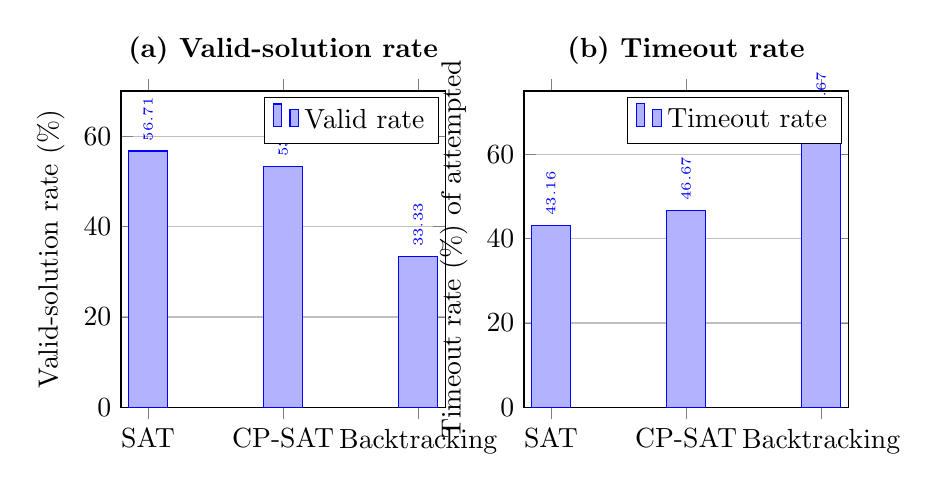
\begin{tikzpicture}
  % ---- Panel (a): valid-solution rate ----
  \begin{axis}[
    name=plotA,
    ybar, bar width=0.5cm, bar shift=0pt,
    symbolic x coords={SAT,CP-SAT,Backtracking},
    xtick=data,
    ylabel={Valid-solution rate (\%)},
    ymin=0, ymax=70,
    ymajorgrids=true,
    title style={font=\bfseries},
    title={(a) Valid-solution rate},
    width=0.47\textwidth, height=5.6cm,
    nodes near coords,
    nodes near coords align={vertical},
    every node near coord/.append style={font=\tiny\bfseries, rotate=90, anchor=west},
  ]
  \addplot coordinates {(SAT,56.71) (CP-SAT,53.33) (Backtracking,33.33)};
  \addlegendentry{Valid rate}
  \end{axis}

  % ---- Panel (b): timeout rate ----
  \begin{axis}[
    at={(plotA.east)}, anchor=west, xshift=1.0cm,
    ybar, bar width=0.5cm, bar shift=0pt,
    symbolic x coords={SAT,CP-SAT,Backtracking},
    xtick=data,
    ylabel={Timeout rate (\%) of attempted},
    ymin=0, ymax=75,
    ymajorgrids=true,
    title style={font=\bfseries},
    title={(b) Timeout rate},
    width=0.47\textwidth, height=5.6cm,
    nodes near coords,
    nodes near coords align={vertical},
    every node near coord/.append style={font=\tiny\bfseries, rotate=90, anchor=west},
  ]
  \addplot coordinates {(SAT,43.16) (CP-SAT,46.67) (Backtracking,66.67)};
  \addlegendentry{Timeout rate}
  \end{axis}
\end{tikzpicture}
\end{document}

\caption{Overall solver-family comparison. Panel (a): valid-solution rate (valid solutions / attempted runs). Panel (b): timeout rate (timeouts / attempted runs). SAT pools seven configurations across 760 attempted runs; CP-SAT and backtracking are single configurations across 120 attempted runs each. SAT's denominator excludes 80 predeclared memory-guard exclusions (pairwise and binary at \(N=81\)). Backtracking's median solve time is not reported (not verified from raw records). All rates are descriptive single measurements with no significance testing.}
\label{fig:overall}
\end{figure}

\subsection{Per-SAT-configuration breakdown}

Table \ref{tab:t2} reports results for each individual SAT configuration. Predeclared exclusions and the live resource-guard rejection are reported separately.

\begin{table}[htbp]
\centering
\caption{Per-SAT-configuration breakdown across all 120 instances. Median solve time is over successful runs only.}
\label{tab:t2}
\small
\begin{tabular}{llcccccccc}
\toprule
Solver & Family & Recorded & Predecl. & Attempted & Valid & Rate (\%) & Timeouts & Guard live & Median (s) \\
\midrule
sat\_pairwise\_cadical153 & SAT & 120 & 40 & 80 & 62 & 77.50 & 18 & 0 & 0.009861 \\
sat\_sequential\_cadical153 & SAT & 120 & 0 & 120 & 62 & 51.67 & 58 & 0 & 0.007760 \\
sat\_binary\_cadical153 & SAT & 120 & 40 & 80 & 60 & 75.00 & 20 & 0 & 0.011180 \\
sat\_commander\_cadical153 & SAT & 120 & 0 & 120 & 63 & 52.50 & 56 & 1 & 0.008905 \\
sat\_product\_cadical153 & SAT & 120 & 0 & 120 & 64 & 53.33 & 56 & 0 & 0.009016 \\
sat\_sequential\_glucose4 & SAT & 120 & 0 & 120 & 60 & 50.00 & 60 & 0 & 0.007728 \\
sat\_sequential\_minisat22 & SAT & 120 & 0 & 120 & 60 & 50.00 & 60 & 0 & 0.006915 \\
\bottomrule
\end{tabular}
\end{table}

The product encoding achieves the most valid solves among SAT configurations (64), matching CP-SAT's total (64). The commander encoding is second (63), with one live resource-guard rejection at \(N=81\). Pairwise and binary show high rates on attempted runs (77.50\%, 75.00\%) only because all 40 of their \(N=81\) instances are predeclared excluded by the memory guard; their rates over all 120 recorded cells would be 51.67\% and 50.00\%, respectively. The differences between product (64), commander (63), and sequential/pairwise (62) are small (one to two solves) and no significance test is performed.

CP-SAT (64 valid on 120 attempted, 53.33\%) matches product's total but is a single configuration; per-configuration SAT comparisons should not be interpreted as a ranking of encoding quality without replication.

\begin{figure}[htbp]
\centering
% ============================================================================
% Figure 3: Per-configuration SAT comparison (valid rate & timeout rate).
% Data source: paper/tables/table2_per_solver_breakdown.csv (audited against
% data/results/benchmark_sat_vs_nonsat.csv).
% Timeout rate computed as timeouts / attempted runs.
% Pairwise and binary each have 40 predeclared N=81 exclusions (attempted=80);
% commander has 1 live resource-guard rejection (attempted=120).
% ============================================================================
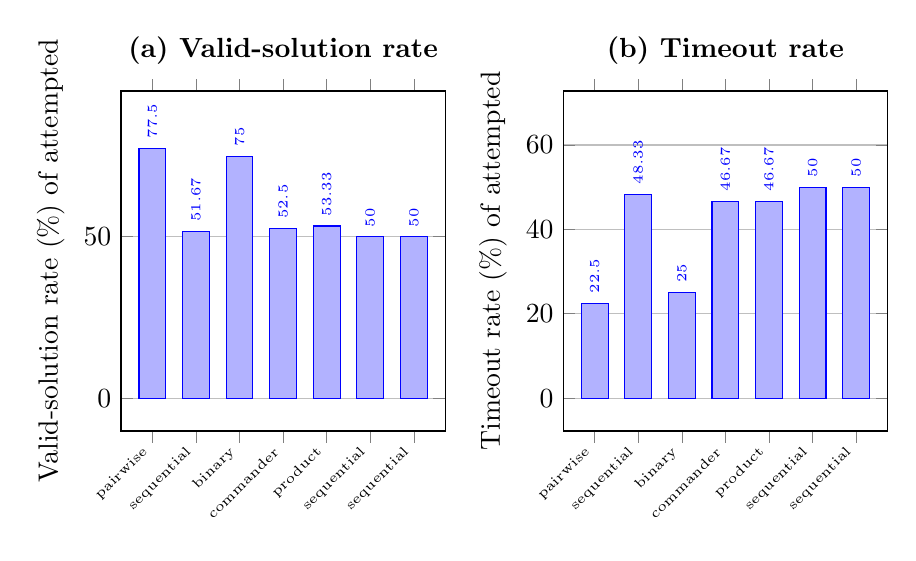
\begin{tikzpicture}
  % ---- Panel (a): valid-solution rate per SAT config ----
  \begin{axis}[
    name=plotA,
    ybar, bar width=0.34cm,
    symbolic x coords={
      pw_cad,seq_cad,bin_cad,com_cad,prod_cad,seq_glu,seq_mini
    },
    xtick=data,
    xticklabels={
      pairwise,sequential,binary,commander,product,sequential,sequential
    },
    xticklabel style={font=\tiny, rotate=45, anchor=east},
    xticklabel style={align=center},
    x tick label style={/pgf/number format/1000 sep={}},
    extra x tick labels={CaDiCaL,CaDiCaL,CaDiCaL,CaDiCaL,CaDiCaL,Glucose,MiniSat},
    extra x tick style={
      xticklabel style={font=\tiny, yshift=1.1em},
      xticklabel pos=right,
    },
    ylabel={Valid-solution rate (\%) of attempted},
    ymin=0, ymax=85,
    ymajorgrids=true,
    enlargelimits=0.12,
    legend style={at={(0.5,-0.42)}, anchor=north, font=\tiny},
    width=0.47\textwidth, height=5.9cm,
    title style={font=\bfseries},
    title={(a) Valid-solution rate},
    nodes near coords,
    nodes near coords align={vertical},
    every node near coord/.append style={font=\tiny\bfseries, rotate=90, anchor=west},
  ]
  \addplot coordinates {(pw_cad,77.50) (seq_cad,51.67) (bin_cad,75.00) (com_cad,52.50) (prod_cad,53.33) (seq_glu,50.00) (seq_mini,50.00)};
  \end{axis}

  % ---- Panel (b): timeout rate per SAT config ----
  \begin{axis}[
    at={(plotA.east)}, anchor=west, xshift=1.5cm,
    ybar, bar width=0.34cm,
    symbolic x coords={
      pw_cad,seq_cad,bin_cad,com_cad,prod_cad,seq_glu,seq_mini
    },
    xtick=data,
    xticklabels={
      pairwise,sequential,binary,commander,product,sequential,sequential
    },
    xticklabel style={font=\tiny, rotate=45, anchor=east},
    xticklabel style={align=center},
    x tick label style={/pgf/number format/1000 sep={}},
    extra x tick labels={CaDiCaL,CaDiCaL,CaDiCaL,CaDiCaL,CaDiCaL,Glucose,MiniSat},
    extra x tick style={
      xticklabel style={font=\tiny, yshift=1.1em},
      xticklabel pos=right,
    },
    ylabel={Timeout rate (\%) of attempted},
    ymin=0, ymax=65,
    ymajorgrids=true,
    enlargelimits=0.12,
    width=0.47\textwidth, height=5.9cm,
    title style={font=\bfseries},
    title={(b) Timeout rate},
    nodes near coords,
    nodes near coords align={vertical},
    every node near coord/.append style={font=\tiny\bfseries, rotate=90, anchor=west},
  ]
  \addplot coordinates {(pw_cad,22.50) (seq_cad,48.33) (bin_cad,25.00) (com_cad,46.67) (prod_cad,46.67) (seq_glu,50.00) (seq_mini,50.00)};
  \end{axis}
\end{tikzpicture}

\caption{Per-SAT-configuration comparison. Panel (a): valid-solution rate of attempted runs. Panel (b): timeout rate of attempted runs. Pairwise and binary each show inflated rates on attempted runs because 40 of their \(N=81\) instances are predeclared excluded by the memory guard (attempted = 80 rather than 120); over all 120 recorded cells their rates would be approximately 51.67\% and 50.00\%. Commander has one live resource-guard rejection. The spread among configurations is small (50.00\%--77.50\% valid on attempted runs) and no significance test is performed.}
\label{fig:satconfigs}
\end{figure}

\subsection{Results by grid size and clue-removal ratio}

Table \ref{tab:t3} reports results by stratum for SAT (pooled across seven configurations), CP-SAT, and backtracking.

\begin{table}[htbp]
\centering
\caption{Results by grid size \(N\) and removal ratio \(r\). Each stratum has 20 instances. SAT attempted runs reflect 7 configurations minus predeclared exclusions at \(N=81\). Median solve time is over successful runs only; ``---'' denotes no valid solves.}
\label{tab:t3}
\small
\begin{tabular}{ccclcccccc}
\toprule
\(N\) & \(r\) & Solver & Attempted & Valid & Rate (\%) & Timeouts & Guard live & Invalid & Median (s) \\
\midrule
9 & 0.5 & SAT & 140 & 140 & 100.00 & 0 & 0 & 0 & 0.008018 \\
9 & 0.5 & CP-SAT & 20 & 20 & 100.00 & 0 & 0 & 0 & 0.003896 \\
9 & 0.5 & Backtracking & 20 & 20 & 100.00 & 0 & 0 & 0 & --- \\
9 & 0.9 & SAT & 140 & 140 & 100.00 & 0 & 0 & 0 & 0.008288 \\
9 & 0.9 & CP-SAT & 20 & 20 & 100.00 & 0 & 0 & 0 & 0.033160 \\
9 & 0.9 & Backtracking & 20 & 20 & 100.00 & 0 & 0 & 0 & --- \\
36 & 0.5 & SAT & 140 & 13 & 9.29 & 127 & 0 & 0 & 6.981681 \\
36 & 0.5 & CP-SAT & 20 & 4 & 20.00 & 16 & 0 & 0 & 7.008288 \\
36 & 0.5 & Backtracking & 20 & 0 & 0.00 & 20 & 0 & 0 & --- \\
36 & 0.9 & SAT & 140 & 138 & 98.57 & 2 & 0 & 0 & 1.508942 \\
36 & 0.9 & CP-SAT & 20 & 20 & 100.00 & 0 & 0 & 0 & 2.270578 \\
36 & 0.9 & Backtracking & 20 & 0 & 0.00 & 20 & 0 & 0 & --- \\
81 & 0.5 & SAT & 100 & 0 & 0.00 & 99 & 1 & 0 & --- \\
81 & 0.5 & CP-SAT & 20 & 0 & 0.00 & 20 & 0 & 0 & --- \\
81 & 0.5 & Backtracking & 20 & 0 & 0.00 & 20 & 0 & 0 & --- \\
81 & 0.9 & SAT & 100 & 0 & 0.00 & 100 & 0 & 0 & --- \\
81 & 0.9 & CP-SAT & 20 & 0 & 0.00 & 20 & 0 & 0 & --- \\
81 & 0.9 & Backtracking & 20 & 0 & 0.00 & 20 & 0 & 0 & --- \\
\bottomrule
\end{tabular}
\end{table}

\textbf{\(N=9\) (standard Sudoku).} All three families achieve 100\% solve rates on both ratios. CP-SAT is faster than SAT at \(r=0.5\) (median 0.0039s vs.\ 0.0080s); SAT is faster than CP-SAT at \(r=0.9\) (median 0.0083s vs.\ 0.0332s, approximately \(4\times\)). Backtracking solves all 40 \(N=9\) instances; exact backtracking medians were not verified from the raw records and are not reported here. These timing differences are single-median comparisons with no significance test; distributions may overlap.

\textbf{\(N=36, r=0.5\) (hardness cliff).} Both SAT (9.29\%) and CP-SAT (20.0\%) fall below 21\%; backtracking solves 0 of 20 (all timeouts). Median valid solve times cluster tightly around 7.0s for SAT and CP-SAT, near the 10s timeout, indicating that successful solves are themselves slow. This stratum represents the most difficult condition tested.

\textbf{\(N=36, r=0.9\) (underconstrained/easy regime).} CP-SAT achieves 100\%; SAT achieves 98.57\% (138/140), with 2 timeouts; backtracking solves 0 of 20. SAT's median (1.51s) is faster than CP-SAT's (2.27s).

\textbf{\(N=81\) (large grid).} Zero valid solutions for all three families across both ratios. SAT pairwise and binary are predeclared excluded (40 per stratum); the remaining five SAT configurations and CP-SAT were attempted and all timed out (99--100 timeouts per SAT stratum plus 1 live guard rejection at \(r=0.5\); 20 timeouts per CP-SAT stratum; 20 timeouts per backtracking stratum). \(N=81\) is intractable within the 10-second timeout for all evaluated approaches; this is a timeout-bound conclusion only, not a claim of unsolvability with larger budgets.

\begin{figure}[htbp]
\centering
% ============================================================================
% Figure 2: Stratified performance by grid size N and removal ratio r.
% Grouped bars of valid-solution rate (%) per solver family across six strata.
% Data source: paper/tables/table3_difficulty_stratification.csv.
% SAT attempted counts reflect 7 configs minus predeclared exclusions at N=81
% (40 per stratum); CP-SAT and Backtracking attempted = 20 per stratum.
% Valid counts: SAT [140,140,13,138,0,0]; CP-SAT [20,20,4,20,0,0];
% Backtracking [20,20,0,0,0,0] across strata
%   (N9r0.5,N9r0.9,N36r0.5,N36r0.9,N81r0.5,N81r0.9).
% Excluded/non-attempted runs are shown as annotations; no bar is drawn for
% missing combinations.
% ============================================================================
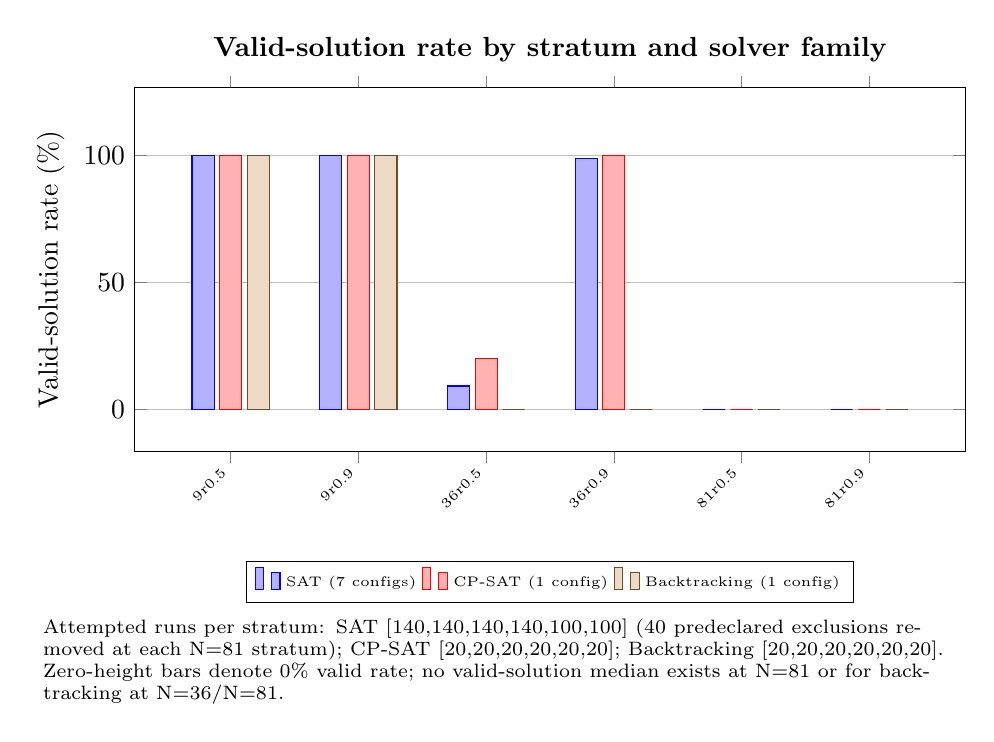
\begin{tikzpicture}
\begin{axis}[
  ybar, bar width=0.28cm,
  symbolic x coords={
    9r0.5,9r0.9,36r0.5,36r0.9,81r0.5,81r0.9
  },
  xtick=data,
  xticklabel style={font=\tiny, rotate=45, anchor=east},
  x tick label style={/pgf/number format/1000 sep={}},
  ylabel={Valid-solution rate (\%)},
  ymin=0, ymax=110,
  ymajorgrids=true,
  enlargelimits=0.15,
  legend style={at={(0.5,-0.30)}, anchor=north, legend columns=3, font=\tiny},
  width=\textwidth, height=6.2cm,
  title style={font=\bfseries},
  title={Valid-solution rate by stratum and solver family},
]
% SAT (pooled 7 configs)
\addplot coordinates {
  (9r0.5,100.00) (9r0.9,100.00) (36r0.5,9.29) (36r0.9,98.57) (81r0.5,0.00) (81r0.9,0.00)
};
\addlegendentry{SAT (7 configs)}
% CP-SAT
\addplot coordinates {
  (9r0.5,100.00) (9r0.9,100.00) (36r0.5,20.00) (36r0.9,100.00) (81r0.5,0.00) (81r0.9,0.00)
};
\addlegendentry{CP-SAT (1 config)}
% Backtracking
\addplot coordinates {
  (9r0.5,100.00) (9r0.9,100.00) (36r0.5,0.00) (36r0.9,0.00) (81r0.5,0.00) (81r0.9,0.00)
};
\addlegendentry{Backtracking (1 config)}
\end{axis}

% Annotation of attempted / excluded counts (placed below axis as a note)
\node[align=left, font=\scriptsize, text width=0.95\textwidth] at (current bounding box.south) [yshift=-0.75cm] {
  Attempted runs per stratum: SAT [140,140,140,140,100,100] (40 predeclared exclusions removed at each N=81 stratum);
  CP-SAT [20,20,20,20,20,20]; Backtracking [20,20,20,20,20,20].
  Zero-height bars denote 0\% valid rate; no valid-solution median exists at N=81 or for backtracking at N=36/N=81.
};
\end{tikzpicture}

\caption{Stratified performance by grid size \(N\) and removal ratio \(r\). Valid-solution rate per solver family across the six strata (20 instances per stratum). SAT pools seven configurations; its attempted count per stratum is 140 at \(N=9\) and \(N=36\), and 100 at \(N=81\) after removing 40 predeclared memory-guard exclusions (pairwise and binary). CP-SAT and backtracking attempt 20 runs per stratum. Zero-height bars denote 0\% valid rate; excluded runs are not drawn as bars but are noted in the caption. SAT's high apparent rates at \(N=81\) are undefined (0 valid / 100 attempted); CP-SAT and backtracking also reach 0\% at \(N=81\). The \(N=36, r=0.5\) stratum is the hardest for all families (below 21\%).}
\label{fig:stratified}
\end{figure}

\subsection{Encoding-size versus runtime}

Per-run \texttt{stats} fields record primary variable count (\(N^3\)), auxiliary variable count (encoding-dependent), total variable count, clause count, and clue count for every SAT run. These data exist in the raw CSV but have not been aggregated or correlated with runtime in this study. The relationship between encoding size and runtime is therefore stated as unanalyzed; no correlation, regression, or significance claim is made. For reference, at \(N=81\): primary variables \(N^3 = 531{,}441\); exactly-one groups \(4N^2 = 26{,}244\); pairwise AMO per group \(N(N-1)/2 = 3{,}240\) clauses (total pairwise AMO clauses \(\approx 85\) million, motivating predeclared exclusion); sequential counter \(N-1=80\) auxiliary variables per group; binary \(\lceil\log_2 81\rceil=7\) auxiliary variables per group.

\begin{figure}[htbp]
\centering
% ============================================================================
% Figure 4: Encoding complexity versus observed outcome (descriptive, no correlation claimed).
% Data source: clause counts computed exactly from src/sudoku/solvers/sat.py
% formulas (groups = 4N^2; per-encoding AMO clauses + one ALO per group + clue units).
% Outcome counts from data/results/benchmark_sat_vs_nonsat.csv (SAT only, 7 configs).
% Panel A: total clauses vs N (log y) for each AMO encoding at N in {9,36,81};
% pairwise and binary at N=81 are marked EXCLUDED (memory guard, ~85M clauses).
% Panel B: stacked outcome counts per stratum (SAT pooled, 7 configs):
% valid vs timeout vs predeclared-excluded vs live-guard-rejection.
% NOTE: runtimes are successful-run-only and timeout-censored; no statistical
% correlation between clause count and runtime has been analyzed.
% ============================================================================
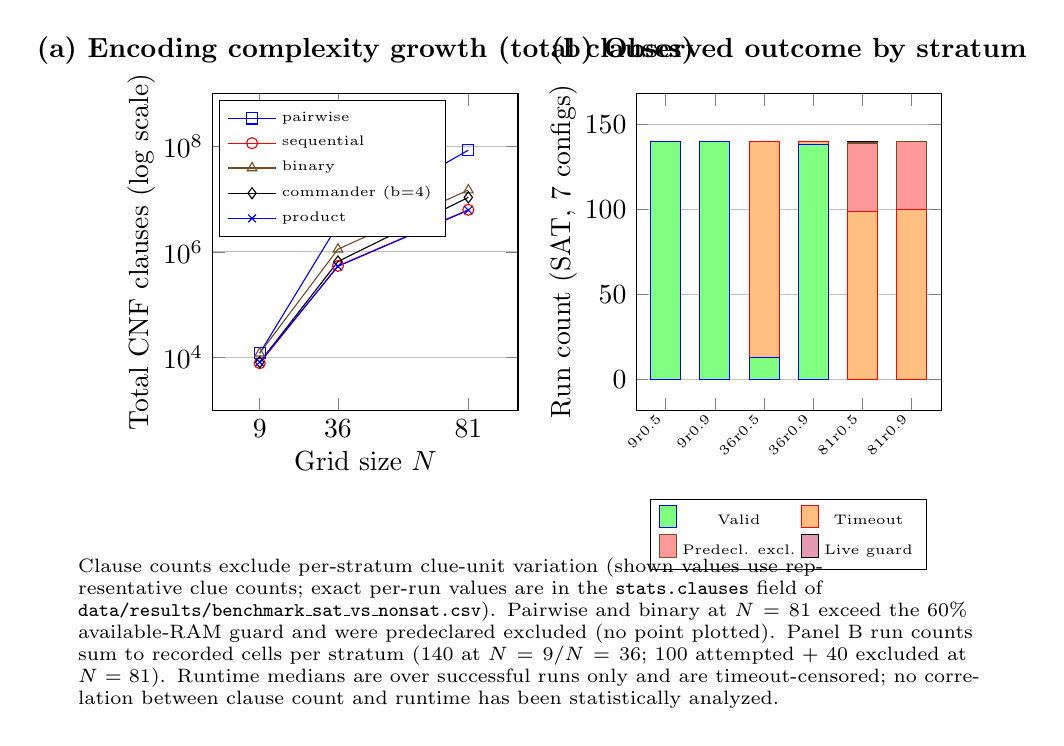
\begin{tikzpicture}
  % ---- Panel A: clause count growth vs N (log scale) ----
  \begin{axis}[
    name=plotA,
    ymode=log,
    ymin=1e3, ymax=1e9,
    xmin=5, xmax=86,
    xtick={9,36,81},
    xlabel={Grid size \(N\)},
    ylabel={Total CNF clauses (log scale)},
    ylabel style={yshift=-0.4em},
    xlabel style={yshift=0.2em},
    ymajorgrids=true,
    title style={font=\bfseries, yshift=0.1em},
    title={(a) Encoding complexity growth (total clauses)},
    width=0.45\textwidth, height=5.6cm,
    legend style={at={(0.02,0.98)}, anchor=north west, font=\tiny, cells={anchor=west}},
    legend columns=1,
    enlarge x limits=0.15,
  ]
  % pairwise: N=9 12028+clues, N=36 ~3.27M, N=81 ~85.06M (excluded)
  \addplot+[mark=square] coordinates {(9,12028) (36,3271144) (81,85056804)};
  \addlegendentry{pairwise}
  % sequential: N=9 7776+clues, N=36 544320, N=81 6298560
  \addplot+[mark=o] coordinates {(9,7776) (36,544320) (81,6298560)};
  \addlegendentry{sequential}
  % binary: N=9 11988+clues, N=36 ~1.12M, N=81 ~14.91M (excluded)
  \addplot+[mark=triangle] coordinates {(9,11988) (36,1124928) (81,14906592)};
  \addlegendentry{binary}
  % commander b=4: N=9 8100+clues, N=36 658368, N=81 ~10.81M
  \addplot+[mark=diamond] coordinates {(9,8100) (36,658368) (81,10812528)};
  \addlegendentry{commander (b=4)}
  % product: N=9 8100+clues, N=36 533952, N=81 ~6.17M
  \addplot+[mark=x] coordinates {(9,8100) (36,533952) (81,6167340)};
  \addlegendentry{product}
  \end{axis}

  % ---- Panel B: stacked outcome counts per stratum ----
  \begin{axis}[
    at={(plotA.east)}, anchor=west, xshift=1.5cm,
    ybar stacked, bar width=0.38cm,
    symbolic x coords={
      9r0.5,9r0.9,36r0.5,36r0.9,81r0.5,81r0.9
    },
    xtick=data,
    xticklabel style={font=\tiny, rotate=45, anchor=east},
    ylabel={Run count (SAT, 7 configs)},
    ylabel style={yshift=-0.4em},
    ymin=0, ymax=150,
    ymajorgrids=true,
    enlargelimits=0.12,
    legend style={at={(0.5,-0.28)}, anchor=north, legend columns=2, font=\tiny},
    width=0.45\textwidth, height=5.6cm,
    title style={font=\bfseries, yshift=0.1em},
    title={(b) Observed outcome by stratum},
  ]
  % valid
  \addplot+[fill=green!50] coordinates {
    (9r0.5,140) (9r0.9,140) (36r0.5,13) (36r0.9,138) (81r0.5,0) (81r0.9,0)
  };
  \addlegendentry{Valid}
  % timeout
  \addplot+[fill=orange!50] coordinates {
    (9r0.5,0) (9r0.9,0) (36r0.5,127) (36r0.9,2) (81r0.5,99) (81r0.9,100)
  };
  \addlegendentry{Timeout}
  % predeclared excluded
  \addplot+[fill=red!40] coordinates {
    (9r0.5,0) (9r0.9,0) (36r0.5,0) (36r0.9,0) (81r0.5,40) (81r0.9,40)
  };
  \addlegendentry{Predecl. excl.}
  % live guard rejection (only N81 r0.5 commander)
  \addplot+[fill=purple!40] coordinates {
    (9r0.5,0) (9r0.9,0) (36r0.5,0) (36r0.9,0) (81r0.5,1) (81r0.9,0)
  };
  \addlegendentry{Live guard}
  \end{axis}

  % ---- Combined annotation below both panels ----
  \node[align=left, font=\scriptsize, text width=0.95\textwidth] at (current bounding box.south) [yshift=-0.8cm] {
    Clause counts exclude per-stratum clue-unit variation (shown values use representative clue counts; exact per-run values
    are in the \texttt{stats.clauses} field of \texttt{data/results/benchmark\_sat\_vs\_nonsat.csv}).
    Pairwise and binary at \(N=81\) exceed the 60\% available-RAM guard and were predeclared excluded (no point plotted).
    Panel B run counts sum to recorded cells per stratum (140 at \(N=9\)/\(N=36\); 100 attempted + 40 excluded at \(N=81\)).
    Runtime medians are over successful runs only and are timeout-censored; no correlation between clause count and runtime
    has been statistically analyzed.
  };
\end{tikzpicture}

\caption{Encoding complexity versus observed outcome (descriptive; no correlation claimed). Panel (a): total CNF clauses versus grid size \(N\) for each AMO encoding, computed exactly from the formulas in \texttt{src/sudoku/solvers/sat.py} (one ALO clause plus AMO clauses per exactly-one group, plus clue-unit clauses). Pairwise and binary at \(N=81\) exceed the 60\% available-RAM memory guard and were predeclared excluded (no data point plotted). Panel (b): observed outcome counts per stratum for SAT (pooled seven configurations), showing valid, timeout, predeclared-excluded, and live-guard-rejection runs. Runtimes are successful-run-only and timeout-censored; no statistical correlation between clause count and runtime has been analyzed. Pairwise/binary at \(N=81\) are excluded rather than timed out, so their runtime performance at that size remains unknown.}
\label{fig:complexity}
\end{figure}

\begin{figure}[htbp]
\centering
% ============================================================================
% Figure 6: Runtime distribution (specification only -- NOT generated).
% Reason: per-run t_total values are recorded in data/results/*.csv but were not
% aggregated under this task's no-code-execution constraint. A meaningful box
% plot / ECDF requires per-run runtime grouped by (family, stratum, config)
% over SOLVED_VALID runs only, which has not been computed.
%
% Specification for a future figure (do not claim generated):
%   - Panel A: Box plot of t_total (seconds, log scale) per stratum per family
%     over SOLVED_VALID runs only. Whiskers exclude censored timeouts.
%   - Panel B: ECDF of t_total for SAT vs CP-SAT vs Backtracking at N=9
%     (the only stratum where all families have successes).
%   - Required fields: t_total, status, N, requested_ratio, solver/encoding/backend.
%   - Disclosure: successful-run-only distributions are affected by timeout
%     censoring (timeouts have no finite runtime and are omitted), inducing
%     survivor bias; medians/percentiles are not comparable to overall completion.
% ============================================================================
\begin{center}
\fbox{\parbox{0.92\textwidth}{
\textbf{Figure 6 (planned): Runtime distribution --- specification only, not generated.}

\textbf{Data required} (all present in the raw CSVs, not yet aggregated):
\texttt{t\_total}, \texttt{status}, \texttt{N}, \texttt{requested\_ratio},
\texttt{solver}, \texttt{encoding}, \texttt{backend} from
\texttt{data/results/benchmark\_sat\_vs\_nonsat.csv} and
\texttt{data/results/backtracking\_results.csv}.

\textbf{Planned panels:}
\begin{itemize}
  \item Panel A --- Box plot of \texttt{t\_total} (seconds, log scale) per stratum
        per solver family over \texttt{SOLVED\_VALID} runs only. Censored timeouts
        omitted (survivor bias disclosed).
  \item Panel B --- ECDF of \texttt{t\_total} at $N=9$ (only stratum where all
        families record successes), comparing SAT (pooled), CP-SAT, backtracking.
\end{itemize}

\textbf{Explicit disclosure:} runtimes are measured over successful runs only;
timeouts contribute to denominators but have no finite runtime. Any distribution
plot is therefore affected by timeout censoring and must not be interpreted as
an overall completion-time distribution. No box plot/ECDF is included in this
manuscript because the per-run aggregation was not performed.
}}
\end{center}

\caption{Planned runtime-distribution figure (specification only; not generated). Per-run \texttt{t\_total} values exist in the raw CSVs but were not aggregated under this task's no-code-execution constraint. A box plot or ECDF over \texttt{SOLVED\_VALID} runs would be affected by timeout censoring (successful-run-only survivor bias) and is therefore not presented as evidence.}
\label{fig:runtimedist}
\end{figure}

\subsection{Data-consistency notes}

Two issues affect the reporting of backtracking results:

\begin{enumerate}
    \item \texttt{data/results/backtracking\_results.csv} contains 120 recorded rows: 40 \texttt{SOLVED\_VALID} (all at \(N=9\), both ratios) and 80 \texttt{TIMEOUT} (all at \(N=36\) and \(N=81\), 40 each), with \texttt{validation\_ok=True} for solved rows and no invalid solutions. These are the backtracking results reported in Section 5.
    \item \texttt{data/results/full\_v1.jsonl} (a preliminary sampled run) contains backtracking runs recorded as \texttt{SOLVER\_ERROR} due to \texttt{TypeError: 'int' object is not iterable} in \texttt{Board.\_\_post\_\_\_init\_\_} (\texttt{src/sudoku\_solver/puzzle.py:64}); the preliminary run was stopped early (\texttt{solver\_error\_rate\_stage}, \texttt{full\_v1\_stop.json}).
\end{enumerate}

These two sources contradict for backtracking. Section 5 reports backtracking from \texttt{backtracking\_results.csv} (40 valid, 80 timeouts), consistent with the totals stated in the task (120 recorded rows, 40 valid, 80 timeouts). The contradiction with \texttt{full\_v1.jsonl} is documented as an unresolved discrepancy in \texttt{docs/paper\_prep/MANUSCRIPT\_EVIDENCE\_AUDIT.md} and \texttt{MANUSCRIPT\_GAPS.md}; no attempt is made to adjudicate which source is correct by re-running code.

\subsection{What is not claimed}

We do not claim: (i) universal superiority of SAT over CP-SAT or backtracking, or vice versa; (ii) that the product encoding is provably the best SAT encoding (its advantage over commander is one solve, 64 vs.\ 63); (iii) statistical significance for any observed difference; (iv) that \(N=81\) Sudoku is unsolvable by any approach (only unsolvable within 10s); (v) a phase transition (the observed difficulty differences lack theoretical or statistical support); or (vi) that classical backtracking in general cannot solve larger Sudoku instances (the timeouts reflect this specific implementation, configured with MRV + forward checking and no AC-3, on the tested instances).

% ============================================================================
% 6. DISCUSSION
% ============================================================================

\section{Discussion}

\subsection{Interpretation of aggregate results}

SAT's 56.71\% valid rate (431/760) and CP-SAT's 53.33\% (64/120) are numerically close, but the comparison is not symmetric. SAT's denominator aggregates seven configurations, so each instance contributes up to seven attempted runs; CP-SAT contributes one. Consequently, SAT's absolute solve count (431) is much larger than CP-SAT's (64) even though the per-attempted-run rates are similar. Per-configuration SAT results range from 50.00\% (sequential with Glucose 4 and MiniSat 2.2) to 77.50\% on attempted runs (pairwise, but with 40 \(N=81\) exclusions). The product encoding's 64 valid solves matches CP-SAT's total, but the one-solve margin over commander (63) is too small to support a ranking claim without replication.

Backtracking's 33.33\% valid rate (40/120) is entirely attributable to \(N=9\), where it solves all 40 instances (median solve time not verified from raw records). Its 0\% at \(N=36\) and \(N=81\) (80 timeouts) reflects this specific implementation's scaling limits on the tested instances, not a general property of classical backtracking. The implementation uses MRV + forward checking without AC-3, LCV, or degree heuristics; stronger configurations were not evaluated.

\subsection{Algorithmic scaling}

At \(N=9\), all three families solve 100\%. At \(N=36, r=0.9\), SAT and CP-SAT remain effective while backtracking times out on all 20 instances. At \(N=36, r=0.5\), all families struggle (below 21\%). At \(N=81\), no family solves any instance within 10s. The empirical difficulty ordering is \(N=9 \ll N=36, r=0.9 < N=36, r=0.5 \ll N=81\), but with only 20 instances per stratum and a single seed, this ordering is descriptive, not generalizable.

The stark contrast between \(r=0.9\) (easy) and \(r=0.5\) (hard) at \(N=36\) is consistent with the intuition that underconstrained puzzles are easier for propagation-driven solvers, while highly constrained puzzles with few clues create large search spaces. However, removal ratio is an experimental condition, not a difficulty label, and the generator documentation explicitly cautions against interpreting \(r\) as difficulty.

\subsection{Representation effects}

SAT's one-hot Boolean encoding with AMO constraints produces large CNFs (hundreds of thousands of variables and millions of clauses at \(N=81\)), which motivated predeclared exclusion of pairwise and binary encodings at \(N=81\). CP-SAT's compact integer-variable model with all-different constraints avoids CNF blow-up but still times out at \(N=81\) within 10s, indicating that the difficulty at \(N=81\) is not solely a formula-size phenomenon. Backtracking's domain-based search scales poorly beyond \(N=9\) on this implementation, consistent with the exponential worst case of backtracking, but the measured timeouts reflect the specific heuristic configuration.

\subsection{Search heuristics}

Backtracking's MRV + forward checking is effective at \(N=9\) (fast solves, exact medians not verified) but insufficient at \(N=36\) and \(N=81\) under the 10s budget. The absence of LCV, degree heuristics, and AC-3 (all confirmed absent from the implementation) may contribute to this scaling limit, but no ablation was performed to isolate their effects. SAT CDCL backends differ (CaDiCaL, Glucose, MiniSat) but their per-configuration results are clustered (50--52\% valid rates for sequential across backends), suggesting backend choice is secondary to encoding and instance difficulty within the tested range.

\subsection{Limits of cross-family comparison}

Comparisons across solver families are limited by (i) different aggregation structures (7 vs.\ 1 vs.\ 1 configurations), (ii) predeclared exclusions affecting only SAT pairwise/binary at \(N=81\), (iii) timeout censoring (timeouts have no finite solve time), and (iv) survivor bias in median solve times (computed over successful runs only, excluding censored timeouts). These limitations are structural to the benchmark design and are disclosed throughout.

% ============================================================================
% 7. THREATS TO VALIDITY
% ============================================================================

\section{Threats to Validity}

\begin{enumerate}
    \item \textbf{Single seed and single automorphism orbit.} All puzzles are generated from base seed 42 and sampled from the automorphism orbit of one base pattern. Results may not generalize to other seeds or grid distributions.
    \item \textbf{Small sample size.} Twenty puzzles per stratum (120 total) limits the precision of solve-rate estimates; no confidence intervals are computed.
    \item \textbf{No replication.} One run per instance per configuration; no variance or reproducibility estimates are available.
    \item \textbf{No confidence intervals or hypothesis tests.} All statistics are descriptive single measurements; no inferential claims are made.
    \item \textbf{Missing environment-lock information.} Hardware (CPU, RAM, OS) is not recorded; \texttt{environment\_lock\_present=false}. Python 3.14.8 is the only confirmed environment detail.
    \item \textbf{Predeclared memory exclusions.} Eighty SAT runs (pairwise and binary at \(N=81\)) are predeclared excluded by the 60\% RAM guard; their performance at \(N=81\) is unknown. This creates an aggregation asymmetry favoring pairwise/binary rates on attempted runs.
    \item \textbf{Timeout censoring and survivor bias.} The 10.0s timeout censors runtimes; medians are computed over successful runs only and exclude censored timeouts, which cluster near the timeout at \(N=36, r=0.5\).
    \item \textbf{Backtracking results are implementation-specific.} Backtracking's 0\% at \(N=36\) and \(N=81\) reflects this implementation (MRV + forward checking, no AC-3/LCV/degree), not classical backtracking generally. A discrepancy exists between \texttt{backtracking\_results.csv} (40 valid, 80 timeouts) and \texttt{full\_v1.jsonl} (backtracking as \texttt{SOLVER\_ERROR}); see Section 5.4 and the audit documents.
    \item \textbf{Three pre-existing failing tests.} \texttt{test\_full\_v1.py} reports three failing tests (the file documents test expectations around matrix shape, resume behavior, and solution-payload preservation). Their impact on result validity has not been established; they are not assumed irrelevant.
    \item \textbf{Two removal ratios only.} \(r \in \{0.5, 0.9\}\); no data for intermediate ratios.
    \item \textbf{Non-unique solutions.} Puzzles may admit multiple valid solutions; correctness is any valid completion matching clues.
    \item \textbf{No commercial solvers.} Gurobi and CPLEX are excluded by license restrictions; their performance is unknown.
    \item \textbf{Limits on external generalization.} Findings apply to the tested dataset, solver versions, timeout, and memory guard only; they do not generalize to other Sudoku distributions, solver configurations, or time budgets.
\end{enumerate}

% ============================================================================
% 8. CONCLUSION
% ============================================================================

\section{Conclusion}

This paper presents an empirical benchmark of SAT (seven configurations, five AMO encodings, three CDCL backends), OR-Tools CP-SAT, and classical backtracking on 120 generalized Sudoku instances (\(N \in \{9, 36, 81\}\); \(r \in \{0.5, 0.9\}\); 20 per stratum) with independent solution validation. Across 1{,}000 attempted runs, SAT achieves 56.71\% (431/760), CP-SAT achieves 53.33\% (64/120), and backtracking achieves 33.33\% (40/120), all with zero invalid solutions. Both SAT and CP-SAT solve 100\% of \(N=9\) instances; all families fall below 21\% at \(N=36, r=0.5\); and no family solves any \(N=81\) instance within the 10-second timeout. The product encoding records the most valid solves among SAT configurations (64), but the margin over commander (63) is one solve and unsupported by significance testing.

The benchmark contributes a documented, reproducible dataset and raw results for replication, explicit accounting of predeclared exclusions and timeout censoring, and descriptive evidence that SAT and CP-SAT are comparable on this benchmark while backtracking's results are confined to \(N=9\) for this implementation.

What remains uncertain: the performance of pairwise and binary SAT encodings at \(N=81\) (predeclared excluded); whether encoding size correlates with runtime (unanalyzed); whether results replicate across seeds or runs; and the exact hardware/software environment. Future studies that would most improve confidence: replication across multiple seeds and puzzle distributions; confidence intervals and hypothesis tests; environment locking; evaluation of backtracking with AC-3, LCV, and degree heuristics; larger time budgets at \(N=81\); and inclusion of the unexecuted \(N=81\) pairwise/binary SAT configurations with sufficient memory.

This is a descriptive, hypothesis-generating benchmark, not a confirmatory study. No claim of publication readiness, universal superiority, or statistical significance is made.

% ============================================================================
% DECLARATIONS
% ============================================================================

\section{Declarations}

\subsection{Funding}

[Author confirmation required: funding sources not documented in the repository.]

\subsection{Competing interests}

[Author confirmation required: competing interests not documented in the repository.]

\subsection{Author contributions}

[Author confirmation required: author contributions not documented in the repository.]

\subsection{Data availability}

Dataset: \texttt{data/manifest.csv} and \texttt{data/puzzles/}. Raw results: \texttt{data/results/benchmark\_sat\_vs\_nonsat.csv} (primary, 960 runs) and \texttt{data/results/backtracking\_results.csv} (backtracking, 120 runs). Dataset metadata: \texttt{data/dataset\_info.json}.

\subsection{Code availability}

Solver implementations: \texttt{src/sudoku/solvers/} (SAT, CP-SAT), \texttt{src/sudoku\_solver/backtracking.py} (backtracking), \texttt{src/sudoku/validator.py} (independent validator), \texttt{src/sudoku/bench/runner.py} (benchmark runner). Table generation: \texttt{scripts/generate\_paper\_tables.py}.

\subsection{Ethical approval}

Not applicable.

% ============================================================================
% REFERENCES
% ============================================================================

\section*{References}
\bibliographystyle{elsarticle-num}
\bibliography{references}

\end{document}
